\section{User Interface Design}
\subsection{Index Page}
This screen is the first thing a user will see when visiting the Monster Mash website. The user will be provided with a link on the menu bar to Login. If they do not have an account, they can create a new one on the Login page too.
\begin{figure*}[h]
\centering
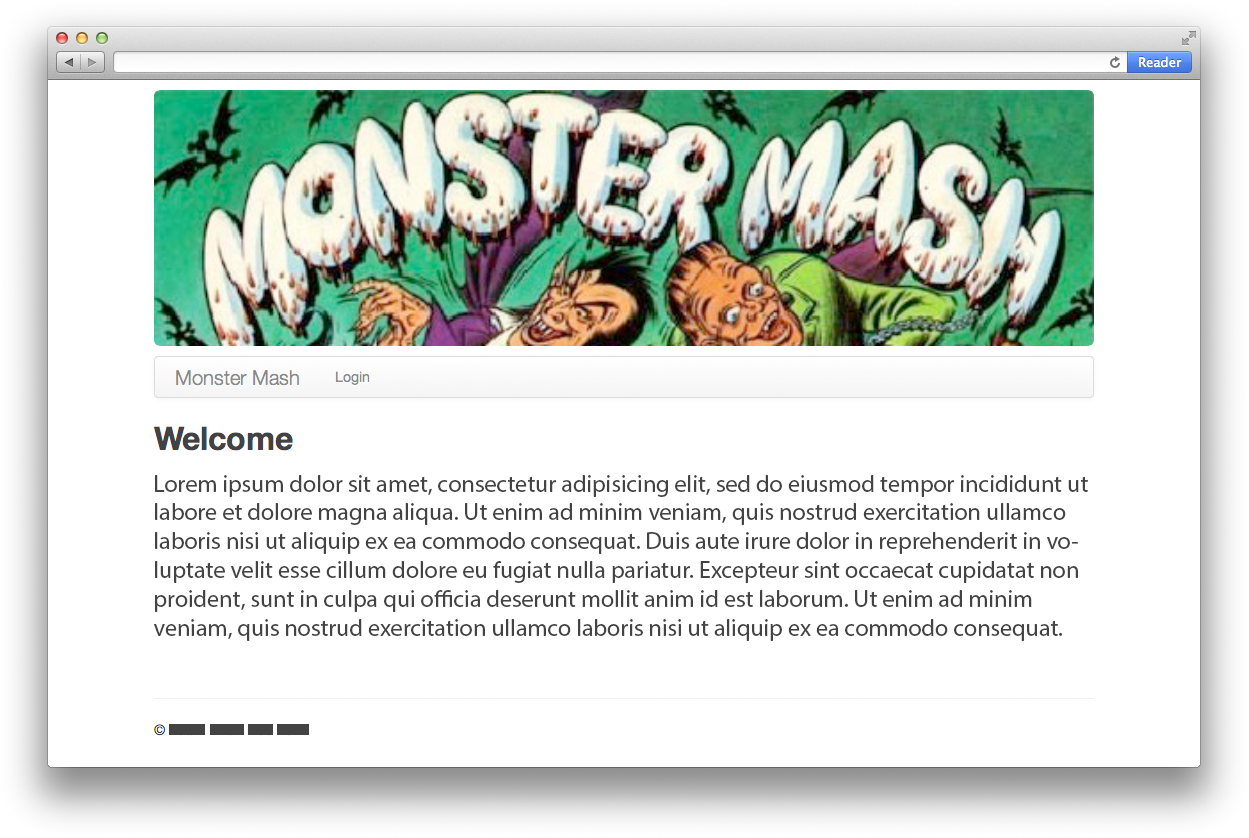
\includegraphics[width=1.00\textwidth]{index.png}
\label{fig:index}
\end{figure*}

\subsection{Login/Register Page}
On this page, a user can login with an existing account or register a new account by clicking on the Register button. This brings up a dialog box ontop of the existing page which lets a user register. Upon successful registration they are brought back to the login page so that they can proceed to login.
\begin{figure*}[h]
\centering
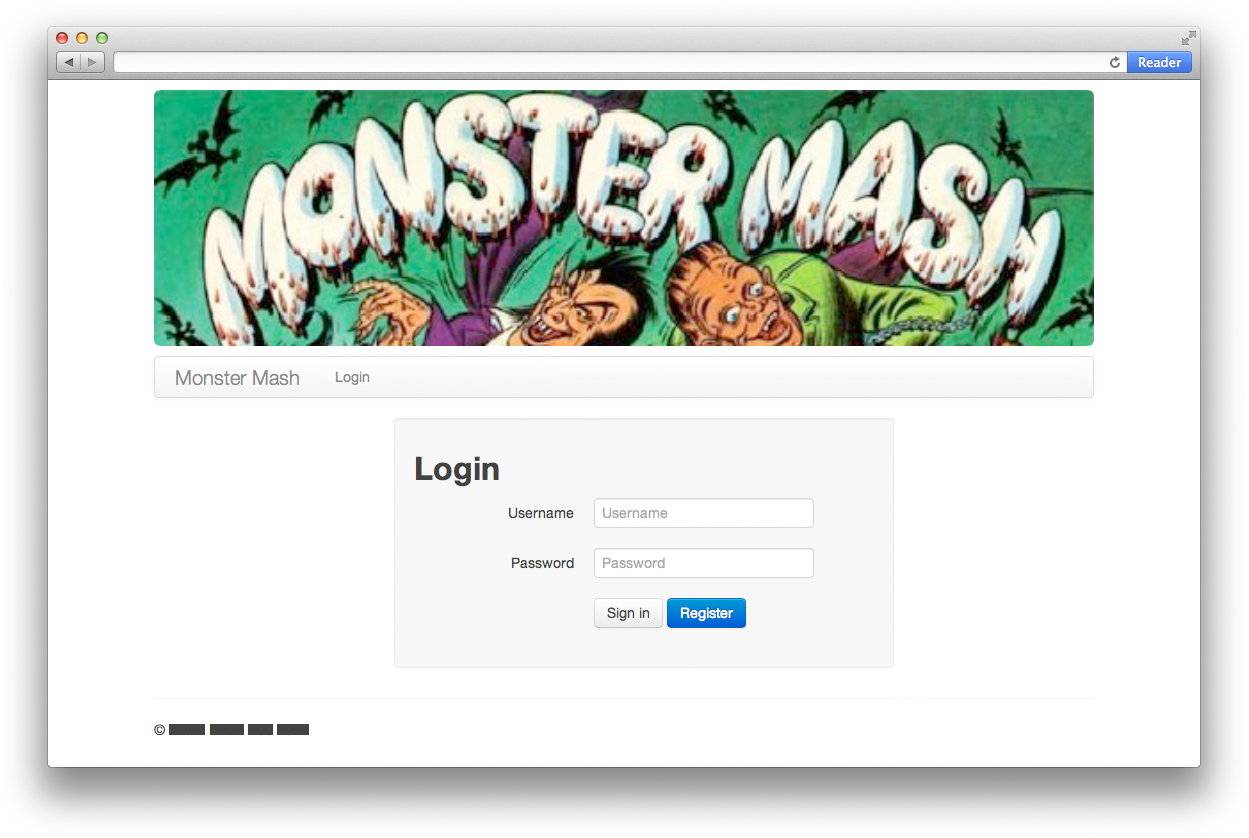
\includegraphics[width=1.00\textwidth]{login.png}
\label{fig:login}
\end{figure*}
\begin{figure*}[h]
\centering
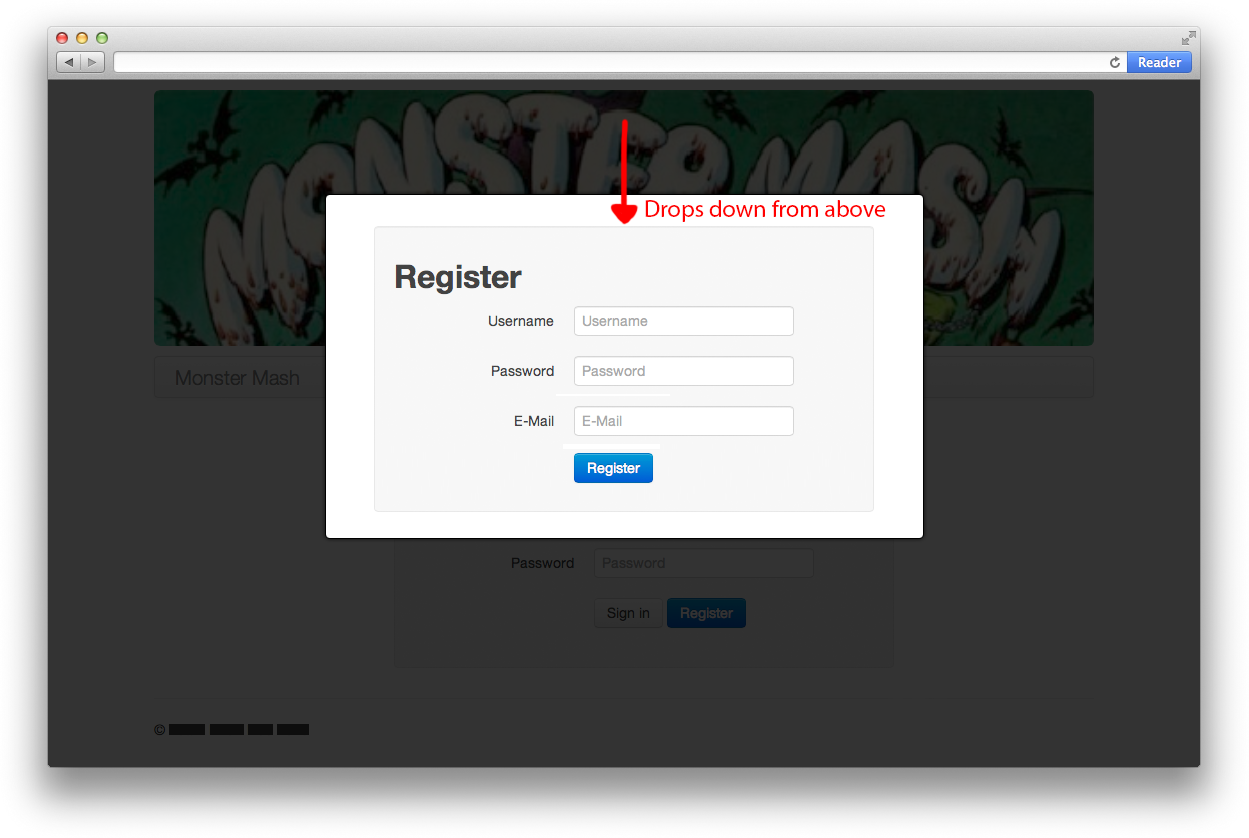
\includegraphics[width=1.00\textwidth]{register.png}
\label{fig:register}
\end{figure*}

\subsection{Home/Add Friend}
This is the page a user sees once they have logged in. The menu bar now has additional links that a user can follow... On the left it shows their personal user stats, and their primary monster's stats. On this page, friend requests, battle requests and other kinds of requests are displayed with an Accept/Decline button.

In the bottom right hand corner is a friends list, to bring up the list of friends, click on it and it slides upwards to display all of the user's friends. If they have none, a message is displayed instead and a button to add friends is displayed. Upon clicking this, a window slides down with fields to add a friend.

When typing in the username box, a list drops down to suggest friend names to add. This list is populated from the user database.
\begin{figure*}[h]
\centering
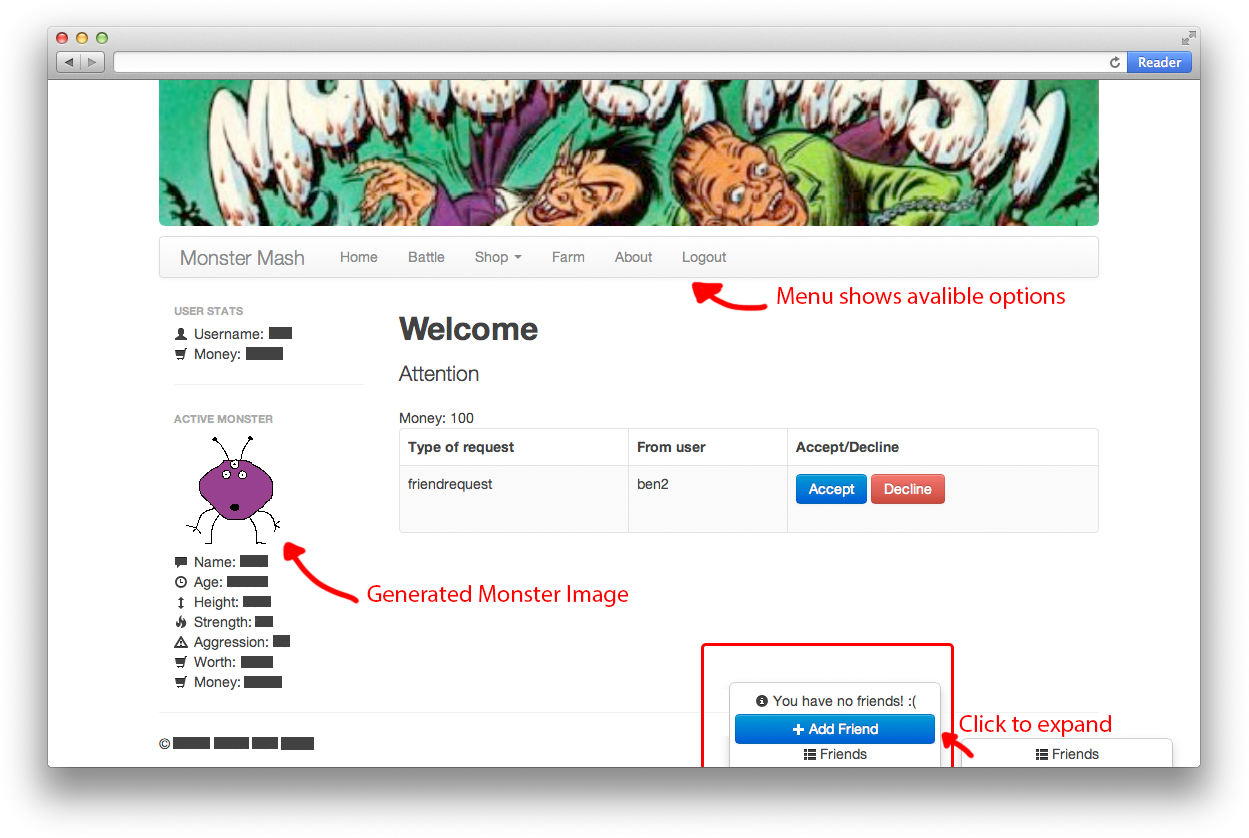
\includegraphics[width=1.00\textwidth]{home.png}
\label{fig:home}
\end{figure*}
\begin{figure*}[h]
\centering
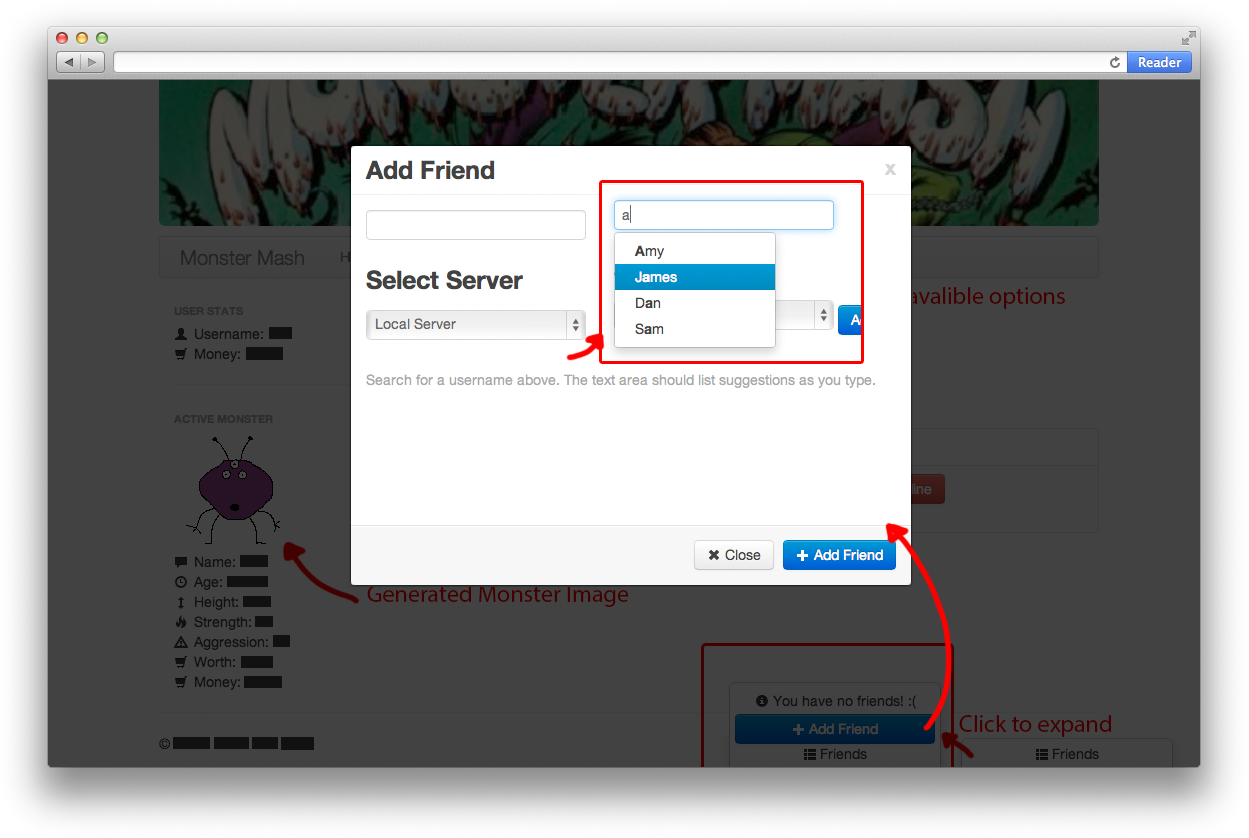
\includegraphics[width=1.00\textwidth]{home_addfriend.png}
\label{fig:home_addfriend}
\end{figure*}

\subsection{Battle Page}
This is the page a user will see when they enter a battle. It shows each monster side by slide, along with their stats, and has a "Battle" button to initiate the battle.
\begin{figure*}[h]
\centering
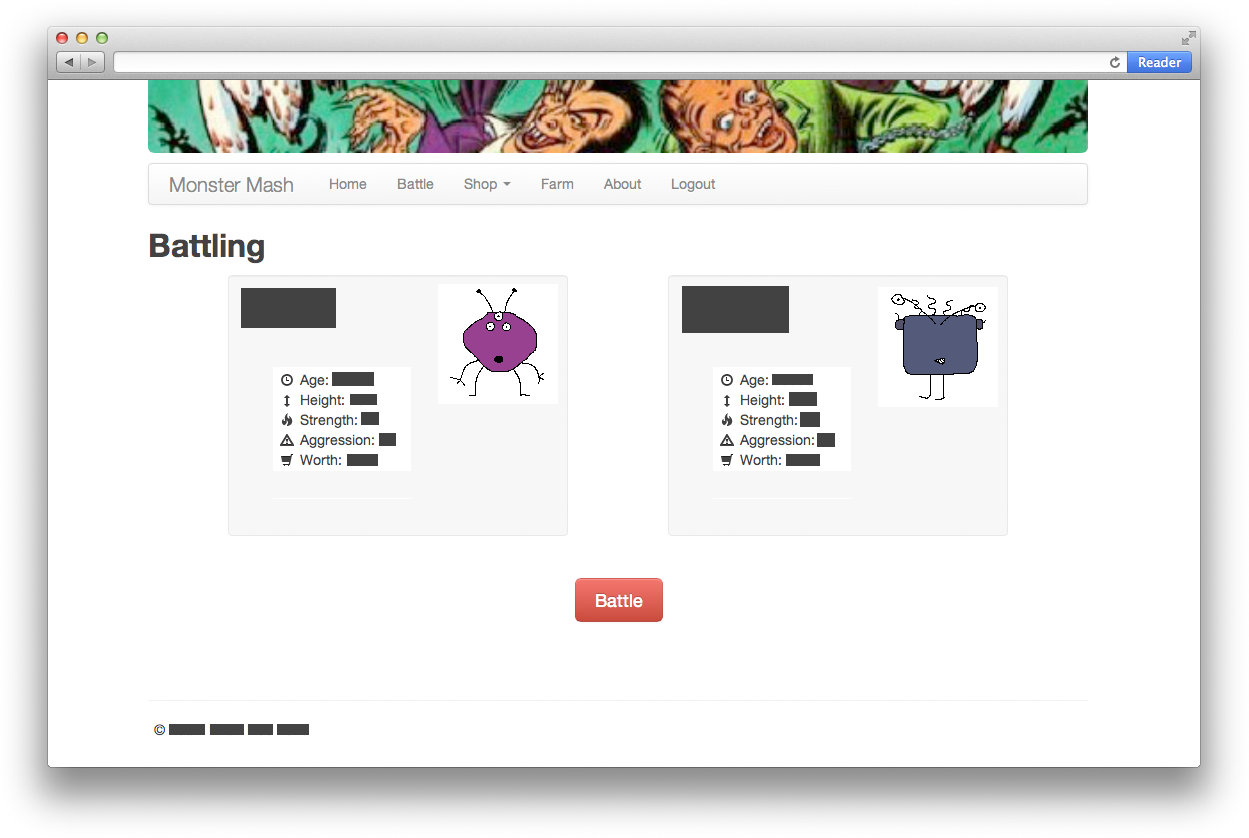
\includegraphics[width=1.00\textwidth]{battle.png}
\label{fig:battle}
\end{figure*}

\subsection{Shop Page}
A user can buy or sell monsters in the shop. Their own monsters will be displayed in a table with an option to sell each of them, or alternatively, a list of unowned monsters can be displayed with an option to buy them. All of the stats are visible in the table so a user knows what they are buying.
\begin{figure*}[h]
\centering
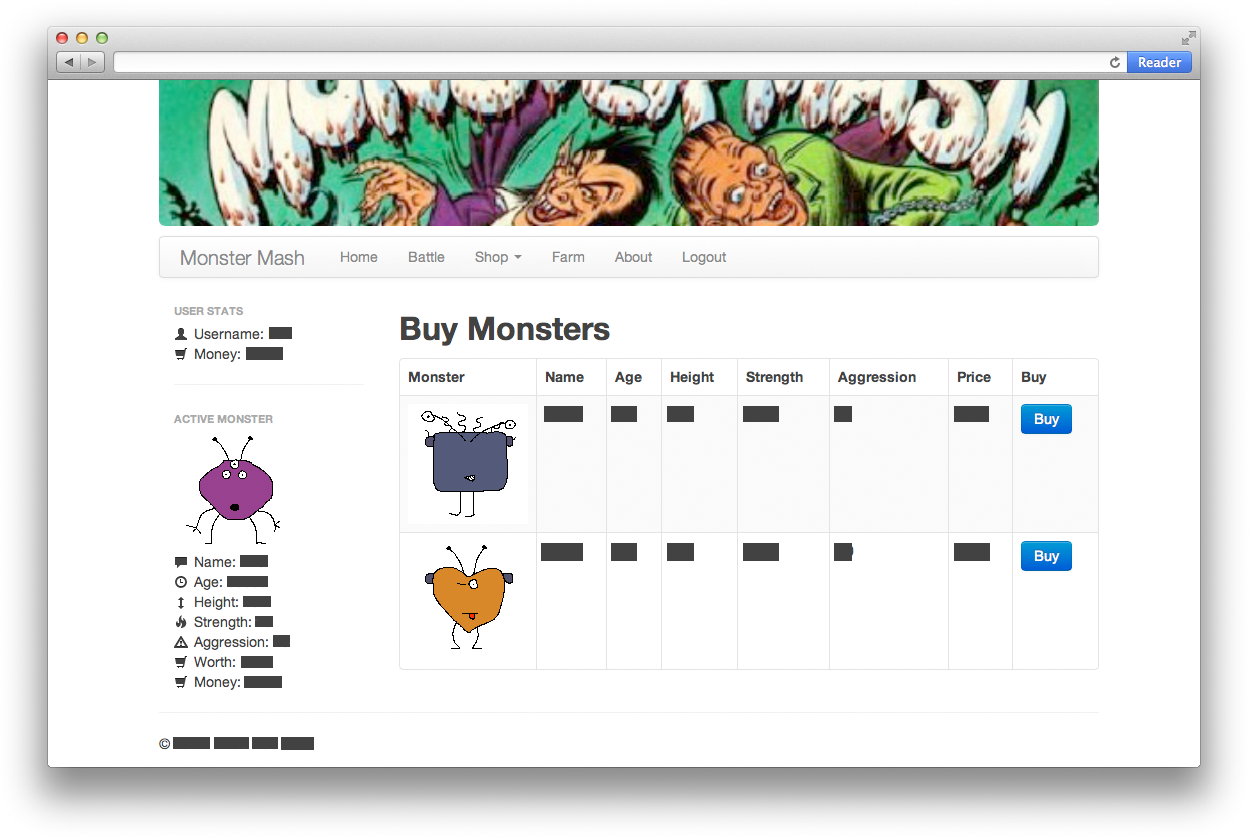
\includegraphics[width=1.00\textwidth]{shop.png}
\label{fig:shop}
\end{figure*}
